\section{Integral ring extension}

See 肖梁

Today, all rings are commutative.

\begin{figure}[H]
\centering
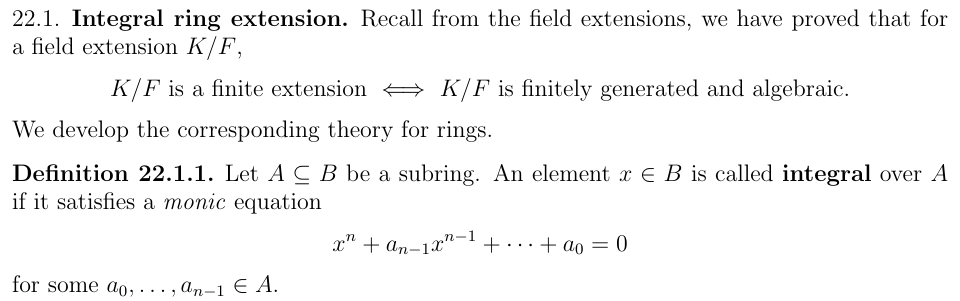
\includegraphics[width=\textwidth]{integral-ring-2025051600.png}
% \caption{}
\label{}
\end{figure}

We point out that, since the polynomial ring over a general ring is no longer a PID, we do not have the notion of “minimal polynomial” here.

\begin{figure}[H]
\centering
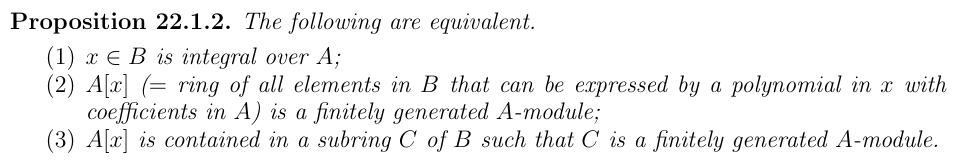
\includegraphics[width=\textwidth]{1-integral-ring-2025051600.png}
% \caption{}
\label{}
\end{figure}

\begin{figure}[H]
\centering
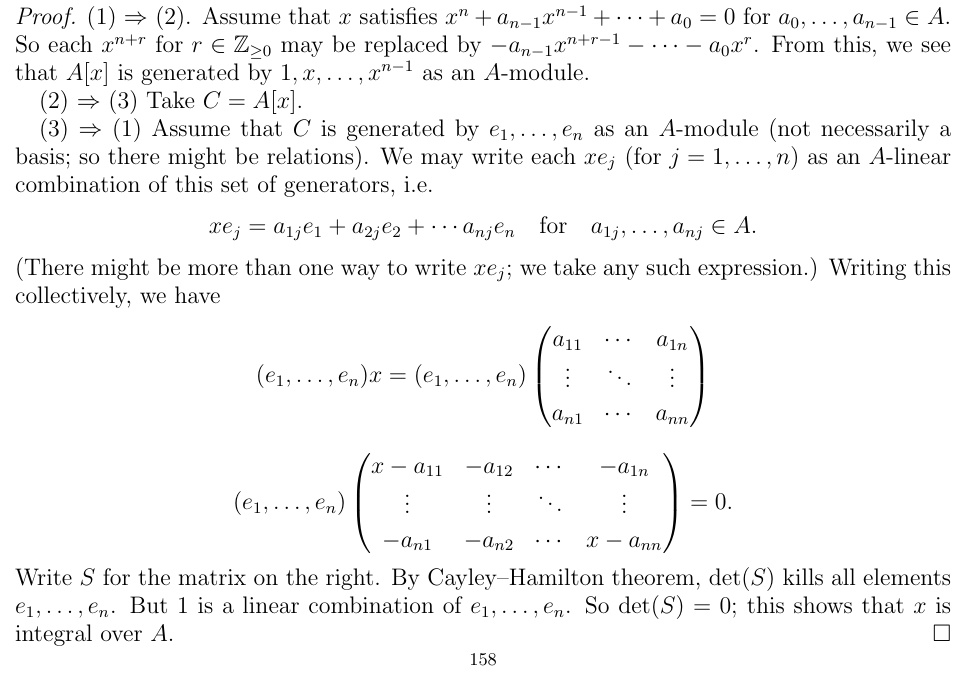
\includegraphics[width=\textwidth]{4-integral-ring-2025051600.png}
% \caption{}
\label{}
\end{figure}

\begin{figure}[H]
\centering
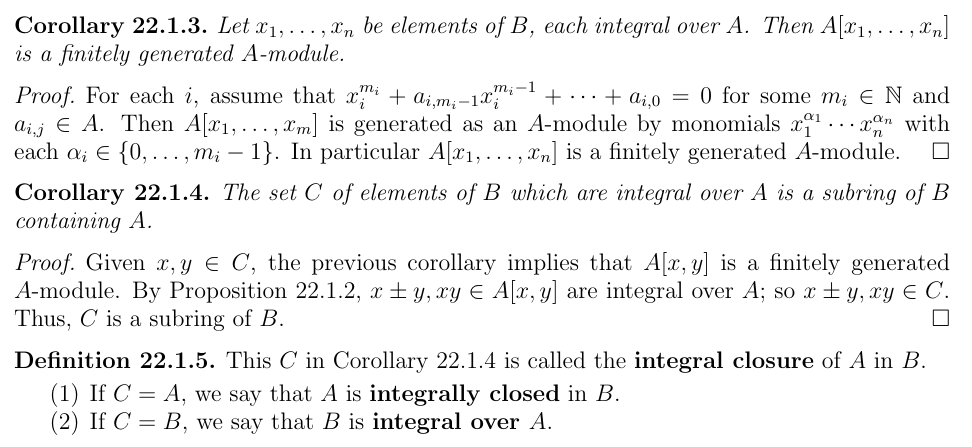
\includegraphics[width=\textwidth]{5-integral-ring-2025051600.png}
% \caption{}
\label{}
\end{figure}
\begin{figure}[H]
\centering
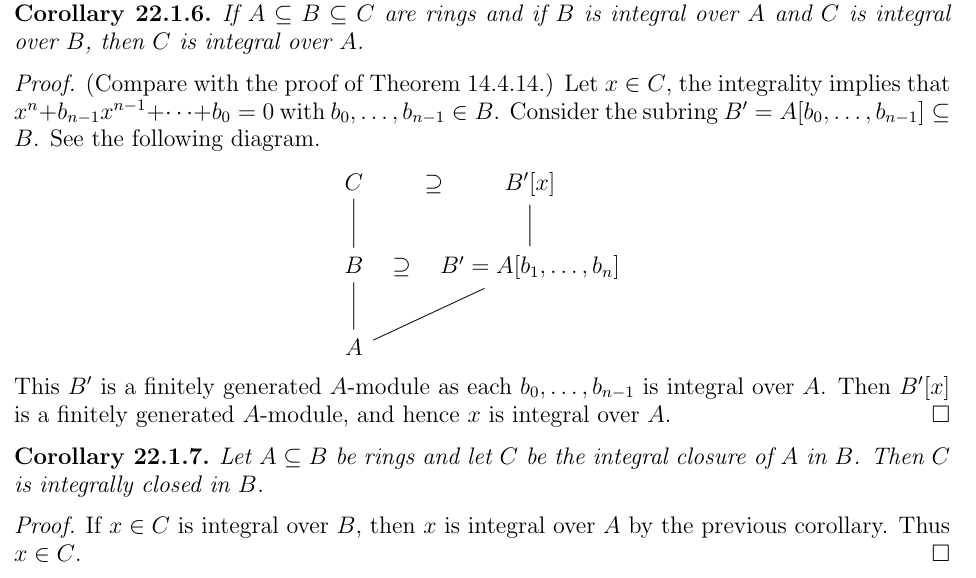
\includegraphics[width=\textwidth]{6-integral-ring-2025051600.png}
% \caption{}
\label{}
\end{figure}

\subsection{Determinant Trick}

\begin{theorem}[The Determinant Trick]
Let $R$ be a commutative ring.
Let $M$ be an $R$-module.
Let $A = (a_{ij})$ be an $n \times n$ matrix with entries $a_{ij} \in R$.
Let $\boldsymbol{v} = \begin{pmatrix} v_1 \\ v_2 \\ \vdots \\ v_n \end{pmatrix}$ be a column vector where each $v_i \in M$.
Suppose that $A \boldsymbol{v} = \boldsymbol{0}$, i.e.,
\[
\sum_{j=1}^{n} a_{ij} v_j = 0 \quad \text{for each } i = 1, \ldots, n
\]
Then, $\det(A) \cdot v_k = 0$ for all $k = 1, \ldots, n$.
In other words, the determinant of the matrix $A$ annihilates each element $v_k$ of the vector $\boldsymbol{v}$.
\end{theorem}
\begin{proof}

\begin{enumerate}
	\item \textbf{Recall the Adjugate Matrix:} For any $n \times n$ matrix $A$ with entries in a commutative ring $R$, its adjugate (or classical adjoint), denoted $\text{adj}(A)$, satisfies the property:
\[
\text{adj}(A) \cdot A = \det(A) \cdot I_n
\]
where $I_n$ is the $n \times n$ identity matrix. The entries of $\text{adj}(A)$ are also in $R$.
	\item \textbf{Multiply the System by the Adjugate:}
We are given the system of equations $A \boldsymbol{v} = \boldsymbol{0}$.
Multiply both sides of this equation on the left by $\text{adj}(A)$:
\[
\text{adj}(A) (A \boldsymbol{v}) = \text{adj}(A) \cdot \boldsymbol{0}
\]
	\item \textbf{Simplify:}
The right side is simply the zero vector:
\[
\text{adj}(A) (A \boldsymbol{v}) = \boldsymbol{0}
\]
Using the associative property of matrix multiplication and the property of the adjugate:
\[
(\text{adj}(A) A) \boldsymbol{v} = \boldsymbol{0}
\]
\[
(\det(A) I_n) \boldsymbol{v} = \boldsymbol{0}
\]
	\item \textbf{Conclusion:}
The product $(\det(A) I_n) \boldsymbol{v}$ is the vector:
\[
\begin{pmatrix} \det(A) & 0 & \cdots & 0 \\ 0 & \det(A) & \cdots & 0 \\ \vdots & \vdots & \ddots & \vdots \\ 0 & 0 & \cdots & \det(A) \end{pmatrix} \begin{pmatrix} v_1 \\ v_2 \\ \vdots \\ v_n \end{pmatrix} = \begin{pmatrix} \det(A) v_1 \\ \det(A) v_2 \\ \vdots \\ \det(A) v_n \end{pmatrix}
\]
Since this vector is equal to the zero vector $\boldsymbol{0}$, each of its components must be zero:
\[
\det(A) \cdot v_k = 0 \quad \text{for all } k = 1, \ldots, n
\]
\end{enumerate}

\end{proof}
This trick is a cornerstone in various proofs in module theory, including versions of Nakayama's Lemma and the Cayley-Hamilton theorem for modules over commutative rings. It elegantly connects the "linear algebra" of matrices over a ring with the structure of modules over that ring.

\begin{definition}[Adjoint of $A$]
Let $A$ be a matrix with entries in a ring $R$. The \textbf{adjoint} of $A$, denoted $\operatorname{adj}(A)$, is the transpose of the matrix of cofactors of $A$.
\end{definition}
In ring theory, the definition of the cofactor of a matrix is analogous to its definition in linear algebra over fields. Let $A$ be an $n \times n$ matrix with entries in a commutative ring $R$.

The $(i, j)$-cofactor of $A$, denoted as $C_{ij}$, is defined as $(-1)^{i+j}$ times the determinant of the $(n-1) \times (n-1)$ matrix formed by deleting the $i$-th row and $j$-th column of $A$.

Specifically:

\begin{enumerate}
	\item Let $A_{ij}$ be the $(n-1) \times (n-1)$ matrix obtained by removing the $i$-th row and the $j$-th column from $A$.
	\item The $(i, j)$-cofactor is $C_{ij} = (-1)^{i+j} \det(A_{ij})$.
\end{enumerate}

The matrix of cofactors is the matrix whose $(i, j)$-entry is $C_{ij}$. The adjugate (or classical adjoint) of $A$, denoted as $\text{adj}(A)$, is the transpose of the cofactor matrix. That is, the $(i, j)$-entry of $\text{adj}(A)$ is $C_{ji}$.
